\documentclass[tikz,margin=.125in]{standalone}
\usetikzlibrary{positioning}
\usetikzlibrary{arrows}
\usetikzlibrary{arrows.meta}
\usetikzlibrary{bending}

\pgfdeclarelayer{bg}
\pgfsetlayers{bg,main}

\begin{document}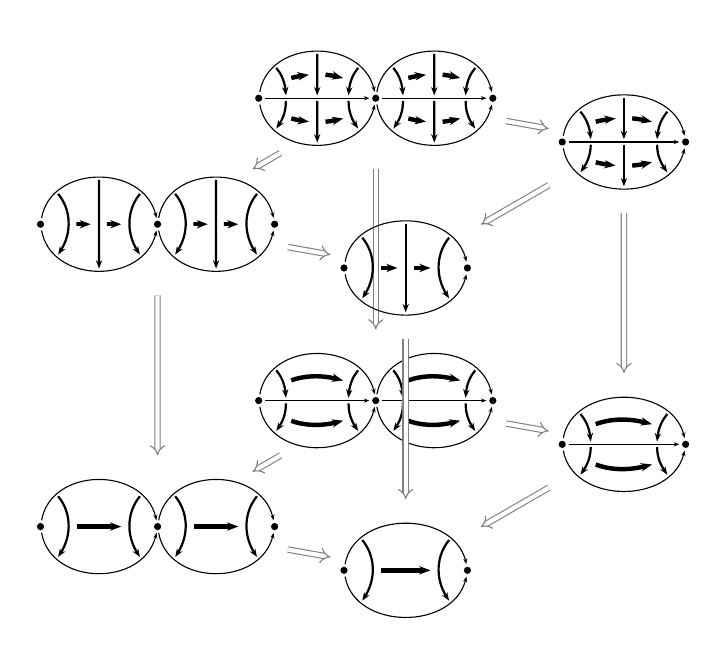
\begin{tikzpicture}[
  0/.append style={
    circle,
    fill,
    node contents={},
    minimum size=3pt-\pgflinewidth,
    inner sep=0,
    outer sep=1pt,
  },
  1/.append style={
    draw,
    ->,
    -{Stealth[length=2pt,bend]},
  },
  2/.append style={
    1, thick,
    shorten <=1pt,
    shorten >=1pt,
    -{Stealth[length=3pt,bend]},
  },
  3/.append style={
    1, ultra thick,
    shorten <=3pt,
    shorten >=3pt,
    -{Stealth[length=4pt,bend]},
  },
  l/.append style={bend left=80,min distance=20pt},
  c/.append style={},
  r/.append style={bend right=80,min distance=20pt},
  s/.append style={pos=.2},
  m/.append style={midway},
  e/.append style={pos=.8},
  V111/.pic={
    \path
      coordinate (O)
      node (00) [0,left=40pt of O]
      node (01) [0]
      node (02) [0,right=40pt of O]
      \foreach \s/\t in {0/1,1/2} {
        (0\s) \foreach \i/\b in {0/l,1/c,2/r}
          {edge [1,\b] coordinate[s](s1\i) coordinate[m](m1\i) coordinate[e](e1\i) (0\t)}
        \foreach \p/\i/\a in {s/0/+1,m/1/+0,e/2/-1} {(\p10) edge [2,out=-90+\a*40,in=90] coordinate[m](m2\i) (\p11)}
        (m20) edge [3,out=0+20,in=180   ] (m21)
        (m21) edge [3,out=0   ,in=180-20] (m22)
        \foreach \p/\i/\a in {s/3/-1,m/4/+0,e/5/+1} {(\p11) edge [2,out=-90,in=90+\a*40] coordinate[m](m2\i) (\p12)}
        (m23) edge [3,out=0-20,in=180   ] (m24)
        (m24) edge [3,out=0   ,in=180+20] (m25)
      }
    ;
  },
  V011/.pic={
    \path
      coordinate (O)
      node (00) [0,left=20pt of O]
      node (01) [0,right=20pt of O]
      (00) \foreach \i/\b in {0/l,1/c,2/r}
        {edge [1,\b] coordinate[s](s1\i) coordinate[m](m1\i) coordinate[e](e1\i) (01)}
      \foreach \p/\i/\a in {s/0/+1,m/1/+0,e/2/-1} {(\p10) edge [2,out=-90+\a*40,in=90] coordinate[m](m2\i) (\p11)}
      (m20) edge [3,out=0+20,in=180   ] (m21)
      (m21) edge [3,out=0   ,in=180-20] (m22)
      \foreach \p/\i/\a in {s/3/-1,m/4/+0,e/5/+1} {(\p11) edge [2,out=-90,in=90+\a*40] coordinate[m](m2\i) (\p12)}
      (m23) edge [3,out=0-20,in=180   ] (m24)
      (m24) edge [3,out=0   ,in=180+20] (m25)
    ;
  },
  V101/.pic={
    \path
      coordinate (O)
      node (00) [0,left=40pt of O]
      node (01) [0]
      node (02) [0,right=40pt of O]
      \foreach \s/\t in {0/1,1/2} {
        (0\s) \foreach \i/\b in {0/l,1/c,2/r}
          {edge [1,\b] coordinate[s](s1\i) coordinate[m](m1\i) coordinate[e](e1\i) (0\t)}
        \foreach \p/\i/\a in {s/0/+1,e/2/-1} {(\p10) edge [2,out=-90+\a*40,in=90] coordinate[m](m2\i) (\p11)}
        (m20) edge [3,out=0+20,in=180-20] (m22)
        \foreach \p/\i/\a in {s/3/-1,e/5/+1} {(\p11) edge [2,out=-90,in=90+\a*40] coordinate[m](m2\i) (\p12)}
        (m23) edge [3,out=0-20,in=180+20] (m25)
      }
    ;
  },
  V110/.pic={
    \path
      coordinate (O)
      node (00) [0,left=40pt of O]
      node (01) [0]
      node (02) [0,right=40pt of O]
      \foreach \s/\t in {0/1,1/2} {
        (0\s) \foreach \i/\b in {0/l,2/r}
          {edge [1,\b] coordinate[s](s1\i) coordinate[m](m1\i) coordinate[e](e1\i) (0\t)}
        \foreach \p/\i/\a in {s/0/+1,m/1/+0,e/2/-1} {(\p10) edge [2,out=-90+\a*40,in=90-\a*40] coordinate[m](m2\i) (\p12)}
        (m20) edge [3,out=0,in=180] (m21)
        (m21) edge [3,out=0,in=180] (m22)
      }
    ;
  },
  V001/.pic={
    \path
      coordinate (O)
      node (00) [0,left=20pt of O]
      node (01) [0,right=20pt of O]
      (00) \foreach \i/\b in {0/l,1/c,2/r}
        {edge [1,\b] coordinate[s](s1\i) coordinate[m](m1\i) coordinate[e](e1\i) (01)}
      \foreach \p/\i/\a in {s/0/+1,e/2/-1} {(\p10) edge [2,out=-90+\a*40,in=90] coordinate[m](m2\i) (\p11)}
      (m20) edge [3,out=0+20,in=180-20] (m22)
      \foreach \p/\i/\a in {s/3/-1,e/5/+1} {(\p11) edge [2,out=-90,in=90+\a*40] coordinate[m](m2\i) (\p12)}
      (m23) edge [3,out=0-20,in=180+20] (m25)
    ;
  },
  V100/.pic={
    \path
      coordinate (O)
      node (00) [0,left=40pt of O]
      node (01) [0]
      node (02) [0,right=40pt of O]
      \foreach \s/\t in {0/1,1/2} {
        (0\s) \foreach \i/\b in {0/l,2/r}
          {edge [1,\b] coordinate[s](s1\i) coordinate[m](m1\i) coordinate[e](e1\i) (0\t)}
        \foreach \p/\i/\a in {s/0/+1,e/2/-1} {(\p10) edge [2,out=-90+\a*40,in=90-\a*40] coordinate[m](m2\i) (\p12)}
        (m20) edge [3,out=0,in=180] (m22)
      }
    ;
  },
  V010/.pic={
    \path
      coordinate (O)
      node (00) [0,left=20pt of O]
      node (01) [0,right=20pt of O]
      (00) \foreach \i/\b in {0/l,2/r}
        {edge [1,\b] coordinate[s](s1\i) coordinate[m](m1\i) coordinate[e](e1\i) (01)}
      \foreach \p/\i/\a in {s/0/+1,m/1/+0,e/2/-1} {(\p10) edge [2,out=-90+\a*40,in=90-\a*40] coordinate[m](m2\i) (\p12)}
      (m20) edge [3,out=0,in=180] (m21)
      (m21) edge [3,out=0,in=180] (m22)
    ;
  },
  V000/.pic={
    \path
      coordinate (O)
      node (00) [0,left=20pt of O]
      node (01) [0,right=20pt of O]
      (00) \foreach \i/\b in {0/l,2/r}
        {edge [1,\b] coordinate[s](s1\i) coordinate[m](m1\i) coordinate[e](e1\i) (01)}
      \foreach \p/\i/\a in {s/0/+1,e/2/-1} {(\p10) edge [2,out=-90+\a*40,in=90-\a*40] coordinate[m](m2\i) (\p12)}
      (m20) edge [3,out=0,in=180] (m22)
    ;
  },
]

\begin{scope}[x={(180-10:1cm)}, y={(90:1.2cm)}, z={(30:1cm)}, scale=3.2]

\node (V000) at (0,0,0) {\tikz\pic{V000};};
\node (V001) at (0,0,1) {\tikz\pic{V001};};
\node (V010) at (0,1,0) {\tikz\pic{V010};};
\node (V011) at (0,1,1) {\tikz\pic{V011};};
\node (V100) at (1,0,0) {\tikz\pic{V100};};
\node (V101) at (1,0,1) {\tikz\pic{V101};};
\node (V110) at (1,1,0) {\tikz\pic{V110};};
\node (V111) at (1,1,1) {\tikz\pic{V111};};

\begin{scope}[
  every edge/.append style={
    -implies,double equal sign distance,gray
  },
]
\draw
 (V111) edge (V011)
 (V110) edge (V111) % ???
 (V011) edge (V001)
 (V011) edge (V010)
 (V101) edge (V001)
 (V100) edge (V101) % ???
 (V110) edge (V010)
 (V110) edge (V100)
 (V100) edge (V000)
 (V010) edge (V000)
 (V001) edge (V000)
;

\begin{pgfonlayer}{bg}
  \draw (V111) edge (V101);
\end{pgfonlayer}

\end{scope}

\end{scope}

\end{tikzpicture}\end{document}
